PuLP is a mathematical modelling language in Python. Using PuLP, a user can quickly and (reasonably) easily define a \ac{MILP} problem and solve it using a variety of solvers including CPLEX, Gurobi and Cbc. As PuLP is built from Python objects it is relatively easy to extend PuLP to use other solvers such as \ac{DIP}. For more details on PuLP see the PuLP project in the COIN-OR repository \cite{coin_or}.

\acf{DIP} \cite{decomp04} provides a framework for solving \ac{MILP} problems using 3 different methods\footnote{The skeleton for a fourth method (branch, relax and cut) exists in \ac{DIP}, but this method is not yet implemented.}: 1) branch and cut; 2) branch, price and cut; and 3) branch, decompose and cut. In this paper we will restrict our attention to 1) and 2).

Branch and cut uses the classic branch-and-bound approach for \ac{MILP} combined with the cutting plane method for removing fractionality in the branch-and-bound nodes' linear programmes. This framework is the basis of many state-of-the-art \ac{MILP} solvers including Gurobi and Cbc. \ac{DIP} provides callback functions for generating user-defined cuts and checking the feasibility of a solution (with respect to the user-defined cuts) within branch and cut. \ac{DIP} also provides a callback function for running a heuristic at each node of the branch-and-bound tree.

Branch, price and cut uses Dantzig-Wolfe decomposition to split a large \ac{MILP} problem into a master problem and one or more subproblems. Branch and cut is used on the master problem. The subproblems solve a pricing problem, defined using the master problem dual values, to add new variables to the master problem.

For branch, price and cut, the cut generation and heuristic callback functions can be used, but extra callback functions enable the user to define their own routines for finding initial variables to include in the master problem and for solving the subproblems to generate new master problem variables. For details on the methods and callback functions provided by \ac{DIP} see \cite{decomp04}.

Dippy extends PuLP to use the \ac{DIP} solver, but it also enables the user-defined routines accessed by the \ac{DIP} callback functions to be implemented in the same Python file as the \ac{MILP} model. Variable scope in Python means that any constraints or variables defined in the \ac{MILP} model are easily accessible in the user-defined routines. Also, \ac{DIP} is implemented so that the \ac{MILP} problem is defined the same way whether branch and cut or branch, price and cut is being used, i.e., it hides the implementation of the master problem and subproblems. This makes it very easy to switch between methods when experimenting with solution methods.

In addition to the \ac{DIP} callback functions (listed in \sbsref{sbs:callbacks}), we have added another callback function that enables user-defined branching in \ac{DIP} and so can be used in any of the solution methods within \ac{DIP}.

\subsection{Callback Functions} \label{sbs:callbacks}

\paragraph{Advanced Branching}
We modified \texttt{chooseBranchVar} in the \ac{DIP} source to become \\ \texttt{chooseBranchSet}. This makes it possible for the user to define:
\begin{itemize}
\item a {\it down} set of variables with (lower and upper) bounds that will be enforced in the down node of the branch; and,
\item an {\it up} set of variables with bounds that will be enforced in the up node of the branch.
\end{itemize}
A typical variable branch on an integer variable $x$ with integer bounds $l$ and $u$ and fractional value $\alpha$ can be implemented by:
\begin{enumerate}
\item choosing the down set to be $\{ x \}$ with bounds $l$ and $\lfloor \alpha \rfloor$;
\item choosing the up set to be $\{ x \}$ with bounds of $\lceil \alpha \rceil$ and $u$.
\end{enumerate}
However, other branching methods may use advanced branching techniques such as the one demonstrated in \scnref{scn:branch}. From \ac{DIP}, {\tt chooseBranchSet} calls \\ {\tt branch\_method} in Dippy.

\paragraph{Customised Cuts} We extended {\tt generateCuts} (in the \ac{DIP} source) to call \\ {\tt generate\_cuts} in Dippy. This enables the user to examine a solution and generate any customised cuts as necessary. We also modified {\tt APPisUserFeasible} to call {\tt is\_solution\_feasible} in Dippy, enabling users to check solutions for feasibility with respect to customised cuts.

\paragraph{Customised Columns (Solutions to Subproblems)} We extended \\ {\tt solveRelaxed} (in \ac{DIP}) to call {\tt relaxed\_solver} in Dippy. This enables the user to utilise the master problem dual variables to produce solutions to subproblems (i.e., columns in the master problem) using customised methods. We also modified {\tt generateInitVars} to call {\tt init\_vars} in Dippy, enabling users to customise the generation of initial columns for the master problem.

\paragraph{Heuristics} We extended {\tt APPheuristics} (\ac{DIP}) to call {\tt heuristics} (Dippy). This enables the user to define customised heuristics at each node in the branch-and-bound tree (including the root node).

\subsection{Interface}

The interface between Dippy (in Python) and DIP (in C++) is summarised in \figref{fig:interface}.
\begin{figure}[htp]
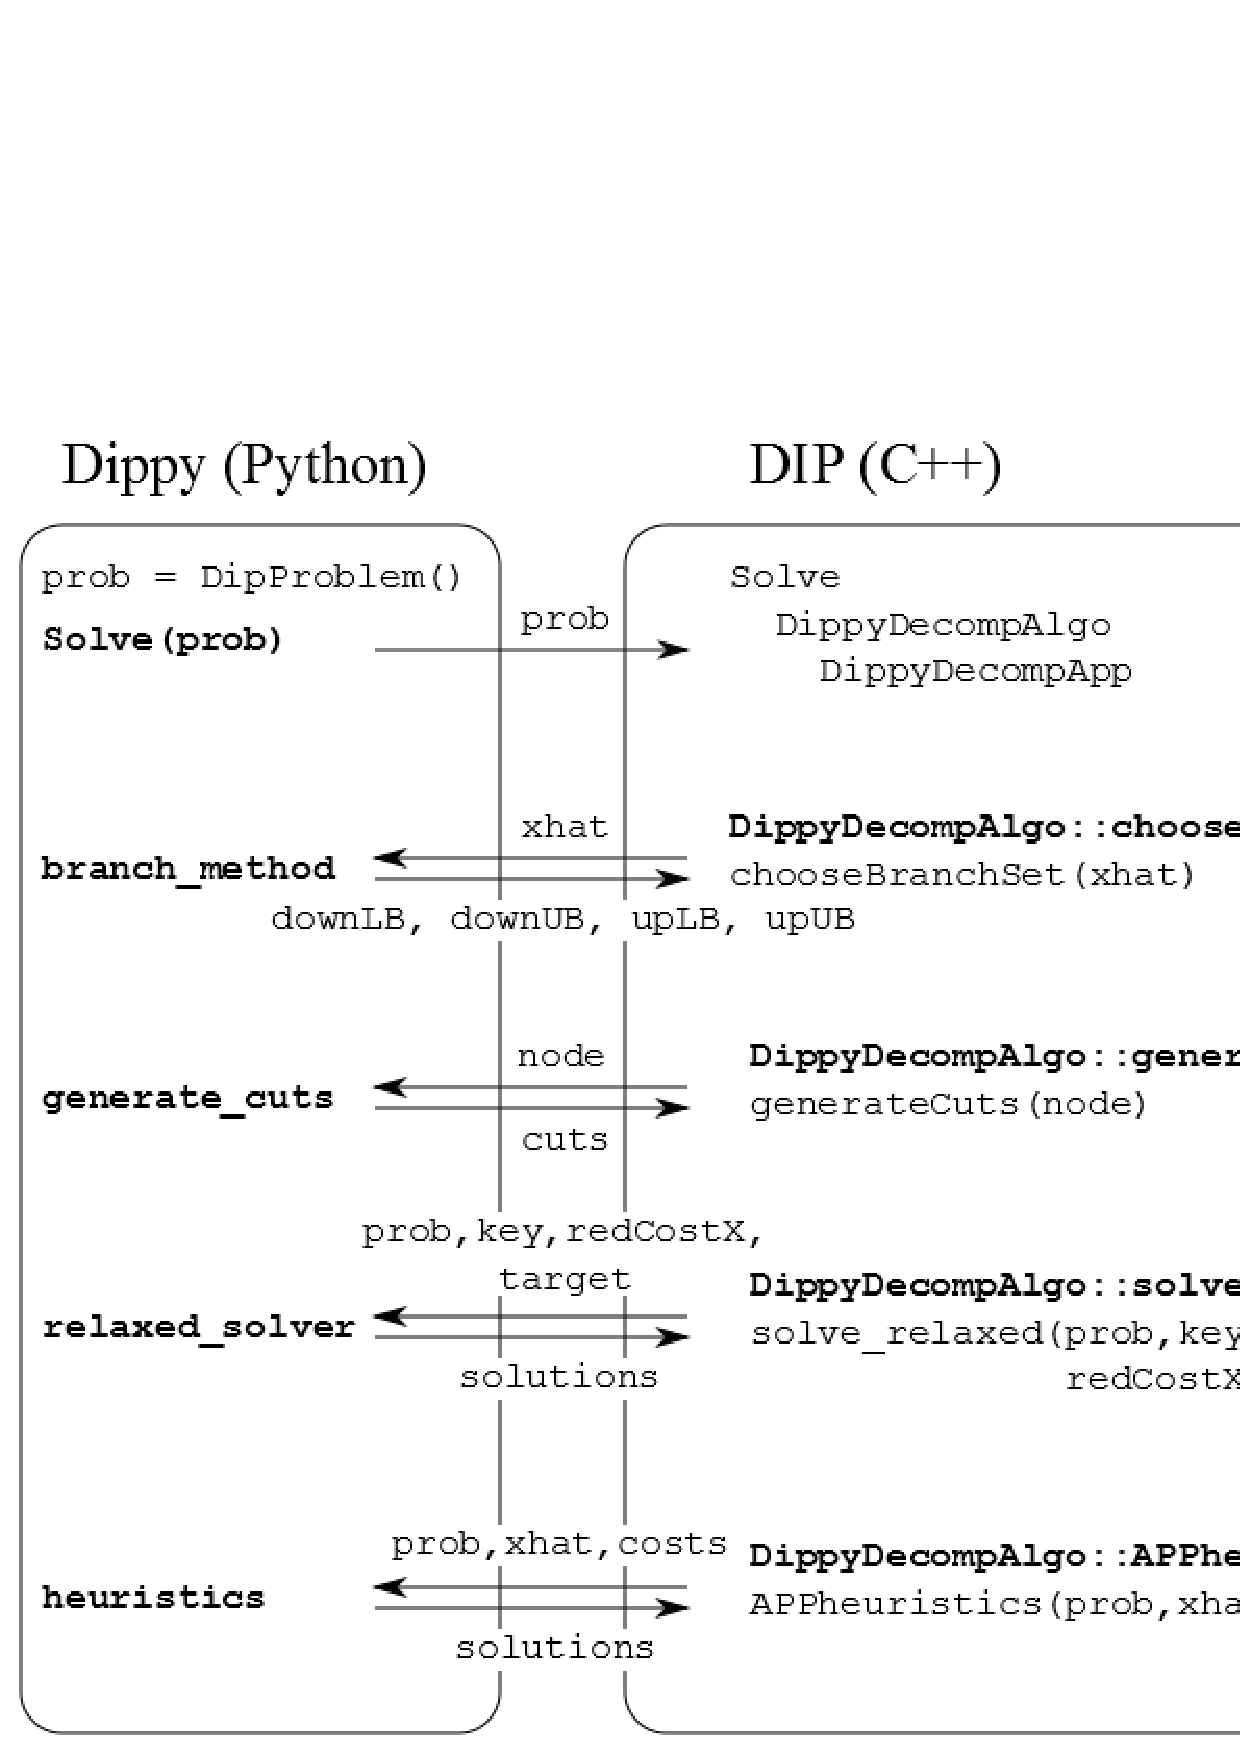
\includegraphics[bb=0 0 960 720,scale=0.45]{interface.png}
\caption{Interface between Dippy and DIP} \label{fig:interface}
\end{figure}

The \ac{MILP} is defined as a {\tt DipProblem} and then solved using the {\tt solve} command in Dippy, that passes the Python {\tt DipProblem} object, {\tt prob}, to DIP in C++. The DIP {\tt solve} creates a {\tt DippyDecompAlgo} object that contains a {\tt DippyDecompApp} object, both of which are populated by data from {\tt prob}. As the DIP {\tt solve} proceeds branches are created by the {\tt DippyDecompAlgo} object using {\tt chooseBranchSet} which passes the current node's fractional solution {\tt xhat} back to the {\tt DipProblem} object {\tt prob}'s {\tt branch\_method} function. This function generates lower and upper bounds for the ``down'' and ``up'' branches and returns to {\tt DippyDecompAlgo::chooseBranchSet}. When DIP generates cuts, it uses the {\tt DippyDecompApp} object's {\tt generateCuts} function which passes the current node's solution {\tt sol} to {\tt prob}'s {\tt generate\_cuts} function. This function generates any customised cuts and returns a list of {\tt cuts} back to \\ {\tt DippyDecompApp::generateCuts}. These interfaces are replicated for the other callback functions provided by Dippy.
